\documentclass[titlepage,letterpaper,final]{scrartcl}

\usepackage{scrindex}           % multiple index support using the "index" package
\usepackage{index}

% This file contains macros included in manual.tex and forcing.tex, in the preamble.
% This way we have all the URLs and such in one place.

%% THE FOLLOWING SHOULD CHANGE FOR A STABLE RELEASE:
\newcommand{\PISMREV}{revision \texttt{@Pism_REVISION_TAG@}}
\newcommand{\PETSCREL}{3.3}
\newcommand{\PISMDOWNLOADMSG}{Get development branch source code:
  \quad \texttt{git clone -b dev git@github.com:pism/pism.git pism-dev} \quad}
\newcommand{\PISMBROWSERURL}{http://www.pism-docs.org/wiki/doku.php?id=browser}
\newcommand{\PISMEMAIL}{\href{mailto:uaf-pism@alaska.edu}{\texttt{uaf-pism@alaska.edu}}}

\newcommand{\normalspacing}{\renewcommand{\baselinestretch}{1.1}\tiny\normalsize}
\newcommand{\tablespacing}{\renewcommand{\baselinestretch}{1.0}\tiny\normalsize}
\normalspacing

\usepackage[usenames,dvipsnames]{xcolor}

\usepackage{bm,url,xspace,verbatim,fancyvrb}
\usepackage{amssymb,amsmath}
\usepackage[pdftex]{graphicx}

\usepackage{booktabs}           % better rules in tables
\usepackage[nohyphen]{underscore}

\newcommand{\ddt}[1]{\ensuremath{\frac{\partial #1}{\partial t}}}
\newcommand{\ddx}[1]{\ensuremath{\frac{\partial #1}{\partial x}}}
\newcommand{\ddy}[1]{\ensuremath{\frac{\partial #1}{\partial y}}}
\renewcommand{\t}[1]{\texttt{#1}}
\newcommand{\Matlab}{\textsc{Matlab}\xspace}
\newcommand{\bq}{\mathbf{q}}
\newcommand{\bU}{\mathbf{U}}
\newcommand{\eps}{\epsilon}
\newcommand{\grad}{\nabla}
\newcommand{\Div}{\nabla\cdot}

%% macros having to do with documentation for options; note these appear in the index

\newindex{default}{idx}{ind}{General Index}
\newindex{options}{odx}{ond}{PISM Command-line options}

\def\optsection#1{%
  \def\optindex##1{\index[options]{#1!##1}}
  \def\optseealso##1{\index[options]{#1|see{##1}}}
}

\optsection{FIXME}

% Use this to index option definitions:
\newcommand{\intextoption}[1]{\texttt{-#1}\optindex{\texttt{-#1}}}

\newcommand{\txtopt}[2]{\texttt{-#1} #2\optindex{\texttt{-#1} #2}}

\newcommand{\listopt}[1]{\txtopt{#1}{\emph{comma-separated list}}}
\newcommand{\fileopt}[1]{\txtopt{#1}{\emph{filename}}}
\newcommand{\timeopt}[1]{\txtopt{#1}{\emph{range or list}}}

\def\variable#1{\texttt{#1}\index{NetCDF variables!\texttt{#1}}}
\def\config#1{\texttt{#1}\index{Configuration flags and parameters!\texttt{#1}}}
\def\class#1{\texttt{#1}\index{C++ classes!\texttt{#1}}}

\DefineVerbatimEnvironment{scriptvrb}{Verbatim}{frame=single,rulecolor=\color{green},framerule=0.1mm,framesep=2mm,xleftmargin=8mm,fontsize=\small}


\usepackage{tikz}
\usetikzlibrary{chains,arrows,shapes}

\addtolength\textheight{0.75in}
\addtolength{\oddsidemargin}{-.4in}
\addtolength{\evensidemargin}{-.4in}
\addtolength{\textwidth}{0.9in}

%% uncomment to see locations of index entries
% \proofmodetrue

% this lets us avoid the scrartcl/hyperref conflict...
\let\ifvtex\relax

\usepackage{xr}
\externaldocument[manual-]{../manual/manual}

% hyperref should be the last package we load
\usepackage[pdftex,
colorlinks=true,
plainpages=false, % only if colorlinks=true
linkcolor=blue,   % only if colorlinks=true
citecolor=blue,   % only if colorlinks=true
urlcolor=blue     % only if colorlinks=true
]{hyperref}

\pdfinfo{
  /Title (PISM climate forcing components)
  /Author (the PISM authors)
  /Subject (Setting up PISM's climate forcing)
  /Keywords (PISM ice sheet modeling climate forcing)
}

\begin{document}

\begin{titlepage}

  \begin{center}
    \vspace*{3.5cm}
    {\huge\usekomafont{title} PISM's climate forcing components}
    \vspace{0.5cm}

    {\Large The PISM Authors}
    \vspace{1cm}
  \end{center}

\setcounter{tocdepth}{3}
\small
\tableofcontents
\normalsize

\vspace{0.3in}

  \begin{center}
    \small Support by email: \PISMEMAIL.

    \medskip
    Please see the \emph{PISM User's Manual} for the full list of authors.

    \medskip
    Manual date \today.  Based on PISM \PISMREV.

    \medskip
    \PISMDOWNLOADMSG
 \end{center}

\vspace{0.3in}
\begin{quote}
  \textsl{Copyright (C) 2004--2016 The PISM Authors}
  \medskip

  \noindent \textsl{This file is part of PISM.  PISM is free software; you can redistribute it and/or modify it under the terms of the GNU General Public License as published by the Free Software Foundation; either version 3 of the License, or (at your option) any later version.  PISM is distributed in the hope that it will be useful, but WITHOUT ANY WARRANTY; without even the implied warranty of MERCHANTABILITY or FITNESS FOR A PARTICULAR PURPOSE.  See the GNU General Public License for more details.  You should have received a copy of the GNU General Public License\index{GPL (\emph{GNU Public License})} along with PISM; see \emph{\texttt{COPYING}}.  If not, write to the Free Software Foundation, Inc., 51 Franklin St, Fifth Floor, Boston, MA  02110-1301 USA}
\end{quote}
\normalsize

\end{titlepage}

\newpage


\section{Introduction}
\label{sec:intro}

PISM has a well-defined separation of climate forcing
from ice dynamics.  This manual is about the climate forcing interface.

By contrast, most options documented in the PISM User's Manual
\footnote{PDF for latest stable release at \url{http://www.pism-docs.org/wiki/lib/exe/fetch.php?media=pism_manual.pdf}.}
control the ice dynamics part.  Section \ref*{manual-sec:climate-inputs} of
the User's Manual does, however, give an overview
of PISM's surface (atmosphere) and ocean (sub-shelf) interfaces.  At
these interfaces the surface mass and energy balances are determined
and/or passed to the ice dynamics code.

\vspace{0.3in}

To get started with climate forcing usage we need to introduce some language to describe parts of PISM.  In this manual a
\emph{component} is a piece of PISM code, usually a C++ class. A combination of
components (or, in some cases, one component) makes up a ``model'' --- an
implementation of a physical/mathematical description of a system.

PISM's climate forcing code has two kinds of components.
\begin{itemize}
\item Ones that can be used as ``stand-alone'' models, such as the
  implementation of the PDD scheme (section~\ref{sec:surface-pdd}). These are
  \emph{model~components}.
\item Ones implementing ``corrections'' of various kinds, such as lapse rate
  corrections (sections~\ref{sec:surface-lapse-rate}
  and~\ref{sec:atmosphere-lapse-rates}) or ice-core derived offsets
  (sections~\ref{sec:atmosphere-delta-temp} and~\ref{sec:delta-sea-level}, for
  example). These are called \emph{modifier~components} or \emph{modifiers}.
\end{itemize}

Model~components and modifiers can be chained as shown in
Figure~\ref{fig:climate-input-data-flow}. For example,
\begin{verbatim}
-ocean constant,delta_SL -ocean_delta_SL_file delta_SL.nc
\end{verbatim}
combines the component providing constant (both in space and time) ocean
boundary conditions with a modifier that
applies scalar sea level (``SL'') offsets. This combination one of the many ocean models that
can be chosen using components as building blocks.

Section~\ref{sec:examples} gives examples of combining components to
choose models.  Before that we address how PISM handles model time
(Section~\ref{sec:model-time}).

\vspace{0.3in}

\begin{quote}
\begin{center}
\emph{Summary of the main idea in using this manual:}
\end{center}

Setting up PISM's climate interface \emph{requires} selecting one surface and one
ocean component. The surface component may use an atmosphere component also;
see Figure \ref{fig:climate-input-data-flow}. Command-line options
\texttt{-atmosphere}, \texttt{-surface} and \texttt{-ocean} each take a
comma-separated list of keywords as an argument; the first keyword \emph{has}
to correspond to a model~component, the rest can be ``modifier'' components.
Any of these options can be omitted to use the default atmosphere, surface or
ocean model~components, but one has to explicitly choose a model~component
to use a modifier. Model~components and modifiers are chained as in Figure
\ref{fig:climate-input-data-flow}.
\end{quote}

\begin{figure}
  \centering
  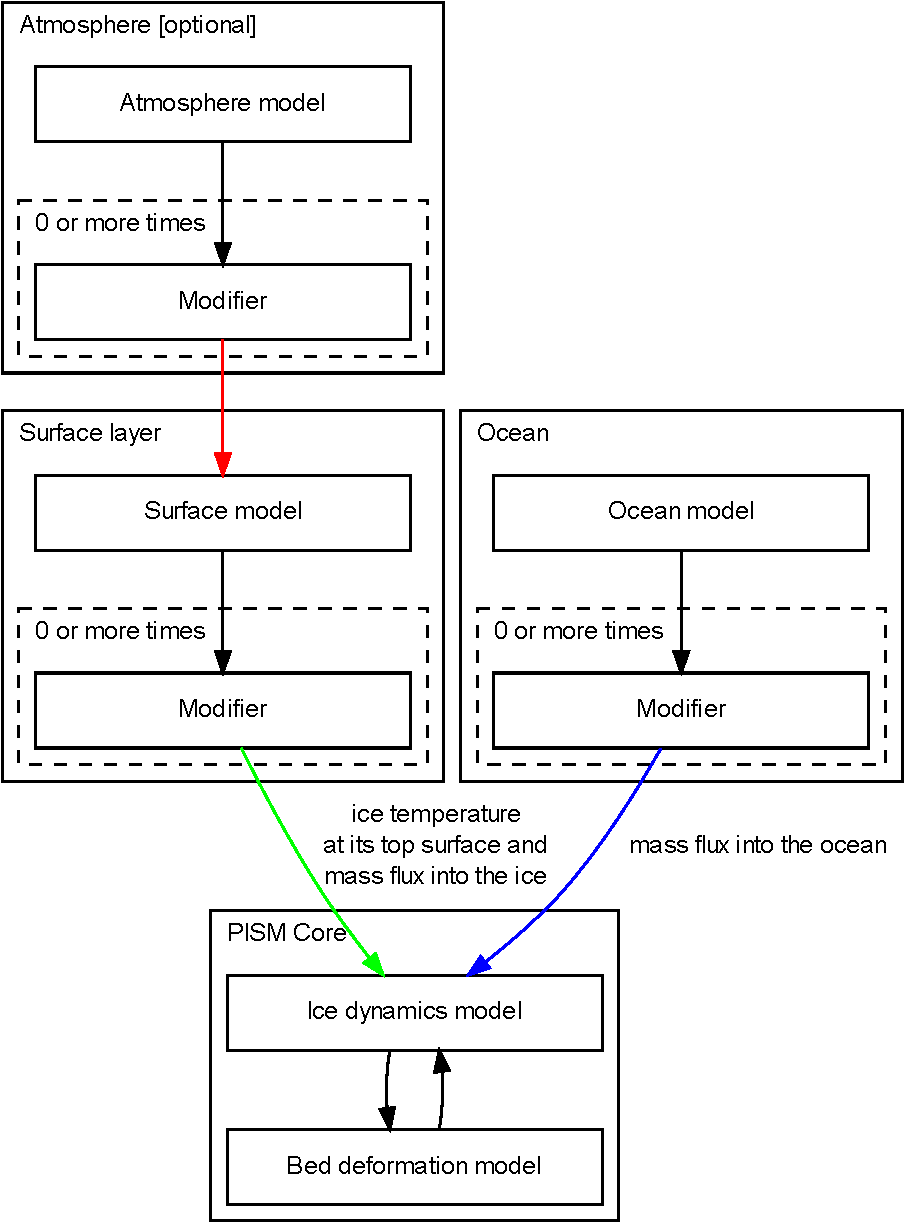
\includegraphics[width=5in]{data-flow.pdf}
  \caption{PISM climate input data flow.  Colored arrows match colored interfaces in
    Figure \ref*{manual-fig:climate-inputs} in the User's Manual.  An atmosphere component is only needed for some surface models.}
  \label{fig:climate-input-data-flow}
\end{figure}


\newpage
\section{Managing model time}
\label{sec:model-time}
\optsection{Managing model time}
\index{Time}

Most of PISM only needs to know how long the current time step is. The
climate forcing (reporting) code, on the other hand, uses time in a
precise manner to provide (and report) the correct values at the right
time. For example: the February mass balance should be used for 28
days (except during leap years) and not $365/12 = 30.4167$ days.




\subsection{Periodic climate data}
\label{sec:periodic-forcing}
\index{Time!periodic}

All components reading time-dependent forcing data from files can interpret
it as ``periodic''.  The length of the period (in years) is specified using
a \texttt{-..._period} option.  For example, to prescribe a periodic climate
which has the same values each year but which includes
inter-annual variations, using the \texttt{-surface given} option, set:
\begin{verbatim}
-surface given -surface_given_period 1 -surface_given_file forcing.nc
\end{verbatim}

Each component has a unique command-line option prefix for a
\texttt{-..._period} option. Please refer to corresponding sections for
allowed prefixes.

If forcing data has the period other than one year it is also
necessary to specify the ``starting time'' using the
\texttt{-..._reference_year} option.

For example, to use a 20 year long climate record as periodic climate starting
at the beginning of the model year 10, do
\begin{verbatim}
-surface given -surface_given_period 20 -surface_given_file forcing.nc \
-surface_given_reference_year 10
\end{verbatim}

Note that the reference year is given in \emph{model years}, not calendar
years.

The \variable{time} variable  in a forcing file that is to  be used as periodic
should start at $0$. (In other words, time in a file with periodic forcing data
is  \emph{time  since   the  beginning  of  a  period}.)   Please  see  section
\ref*{manual-sec:calendars}  of the User's Manual for a  discussion  of time  units  appropriate in  forcing
files.


\subsection{Using time bounds in forcing data}
\label{sec:time-bounds}
\index{Time!bounds}

PISM interprets climate forcing data as piecewise-constant in time. A forcing
file is required to contain time bounds corresponding to each record.

PISM follows the CF (Climate and Forecasting) meta-data conventions. The
\texttt{ncdump -h} output from a conforming file would look similar to:
\begin{verbatim}
netcdf forcing {
dimensions:
        time = UNLIMITED ; // (214 currently)
        nv = 2 ;
variables:
        double time(time) ;
                time:units = "seconds since 2000-1-1" ;
                time:axis = "T" ;
                time:bounds = "time_bounds" ;
                time:calendar = "gregorian" ;
                time:long_name = "time" ;
        double nv(nv) ;
        double time_bounds(time, nv) ;
\end{verbatim}

The \variable{time_bounds} variable stores the starting and the ending time for
each interval in the forcing. This variable is assumed to have the same units
as the \variable{time} variable it is associated with, which is why its arguments
are not set in this example.

Please see the
\href{http://cf-pcmdi.llnl.gov/documents/cf-conventions/1.6/cf-conventions.html#cell-boundaries}{CF
Conventions} document for details.




\clearpage\newpage
\section{Examples and corresponding options}
\label{sec:examples}

This section gives a very brief overview of some coupling options. Please see sections referenced below for more information.

\subsection{One way coupling to a climate model}
\label{sec:one-way-coupling}
\index{One-way coupling to a climate model}

One-way coupling of PISM to a climate model can be achieved by reading a NetCDF
file with time- and space-dependent climate data produced by a climate model.

There are two cases:
\begin{itemize}
\item coupling to a climate model that includes surface (firn, snow) processes
\item coupling to a climate model providing near-surface air temperature and precipitation
\end{itemize}

\subsubsection{Reading ice surface temperature and mass balance}
\label{sec:ice-surface-bc}

This is the simplest case.  It is often the preferred case, for example when
the climate model in use has high quality surface mass and energy sub-models
which are then preferred to the highly simplified (e.g.~temperature index)
surface models in PISM.

\begin{center}
  \begin{tabular}{lp{0.7\textwidth}}
    \toprule
    Variable names: & \variable{climatic_mass_balance}, \variable{ice_surface_temp} \\
    Options: & \texttt{-surface given -surface_given_file forcing.nc} \\
    See also & \ref{sec:surface-given} \\
    \bottomrule
  \end{tabular}
\end{center}

\subsubsection{Reading air temperature and precipitation}
\label{sec:air-temp-and-precip}

As mentioned above, if a climate model provides near-surface air temperature
and precipitation, these data need to be converted into top-of-the-ice
temperature and climatic mass balance.

One way to do that is by using a temperature index (PDD) model~component included in
PISM. This component has adjustable parameters; default values come
from~\cite{RitzEISMINT}.

\begin{center}
  \begin{tabular}{lp{0.7\textwidth}}
    \toprule
    Variable names: & \variable{precipitation}, \variable{air_temp} \\
    Options: & \texttt{-atmosphere given -atmosphere_given_file forcing.nc -surface~pdd} \\
    See also & \texttt{-atmosphere given}: \ref{sec:atmosphere-given},\\
    &\texttt{-surface pdd}: \ref{sec:surface-pdd} \\
    \bottomrule
  \end{tabular}
\end{center}

If melt is negligible \texttt{-surface pdd} should be replaced with \texttt{-surface simple} (see section~\ref{sec:surface-simple}).

\subsection{Using climate anomalies}
\label{sec:use-case-climate-anomalies}

Prognostic modeling experiments frequently use time- and space-dependent
air temperature and precipitation anomalies.

\begin{center}
  \begin{tabular}{lp{0.7\textwidth}}
    \toprule
    Variable names: & \variable{precipitation_anomaly}, \variable{air_temp_anomaly}\\
    Options:  & \texttt{\mbox{-atmosphere given,anomaly}
      \mbox{-atmosphere_anomaly_file anomalies.nc}
      \mbox{-surface simple}
    } \\
    See  also   &  \texttt{-atmosphere~given}: \ref{sec:atmosphere-given}, \\
    & \texttt{anomaly}: \ref{sec:atmosphere-anomaly}, \\
    & \texttt{-surface~simple}: \ref{sec:surface-simple} \\
    \bottomrule
  \end{tabular}
\end{center}

The \texttt{simple} surface model~component re-interprets precipitation as
climatic mass balance, which is useful in cases when there is no melt
(Antarctic simulations is an example).

Simulations of the Greenland ice sheet typically use \texttt{-surface~pdd} instead of \texttt{-surface~simple}.

\subsection{SeaRISE-Greenland}
\label{sec:use-case-searise-greenland}

The SeaRISE-Greenland setup uses a parameterized near-surface air temperature
\cite{Faustoetal2009} and a constant-in-time precipitation field read from an
input (\texttt{-i}) file. A temperature-index (PDD)
scheme is used to compute the climatic mass balance.

\begin{center}
  \begin{tabular}{lp{0.7\textwidth}}
    \toprule
    Variable names: & \variable{precipitation}, \variable{lat}, \variable{lon} \\
    Options: & \texttt{-atmosphere searise_greenland -surface~pdd} \\
    See also & \texttt{-atmosphere searise_greenland}: \ref{sec:atmosphere-searise-greenland},\\
    &\texttt{-surface pdd}: \ref{sec:surface-pdd} \\
    \bottomrule
  \end{tabular}
\end{center}

The air temperature parameterization is a function of latitude
(\variable{lat}), longitude (\variable{lon}) and surface elevation (dynamically
updated by PISM).

\subsection{SeaRISE-Greenland paleo-climate run}
\label{sec:use-case-searise-greenland-paleo}

The air temperature parameterization in the previous section is appropriate for
present day modeling. PISM includes some mechanisms allowing for corrections
taking into account differences between present and past climates. In
particular, one can use ice-core derived scalar air temperature offsets
\cite{JohnsenetalGRIP}, precipitation adjustments~\cite{Huybrechts02}, and sea
level offsets from SPECMAP~\cite{Imbrieetal1984}.

\begin{center}
  \begin{tabular}{lp{0.7\textwidth}}
    \toprule
    Variable names: & \variable{precipitation}, \variable{delta_T},
    \variable{delta_SL}, \variable{lat}, \variable{lon}\\
    Options: & \texttt{\mbox{-atmosphere searise_greenland,delta_T}
      \mbox{-atmosphere_delta_T_file delta_T.nc}
      \mbox{-surface pdd}
      \mbox{-ocean constant,delta_SL}
      \mbox{-ocean_delta_SL_file delta_SL.nc}
    } \\
    See also & \texttt{-atmosphere searise_greenland}:
    \ref{sec:atmosphere-searise-greenland}, \\
    & \texttt{-surface pdd}: \ref{sec:surface-pdd} \\
    & \texttt{-ocean constant}: \ref{sec:ocean-constant} \\
    & \texttt{delta_SL}: \ref{sec:delta-sea-level} \\
    \bottomrule
  \end{tabular}
\end{center}

Note that the temperature offsets are applied to \emph{air} temperatures at the
\emph{atmosphere level}. This ensures that $\Delta T$ influences the PDD
computation.

\subsection{Antarctic paleo-climate runs}
\label{sec:use-case-antarctica-paleo}

\begin{center}
  \begin{tabular}{lp{0.7\textwidth}}
    \toprule
    Variable names: & \variable{climatic_mass_balance},
    \variable{air_temp}, \variable{delta_T}, \variable{delta_SL}\\
    Options: & \texttt{\mbox{-surface given,delta_T}
      \mbox{-surface_delta_T_file delta_T.nc}
      \mbox{-ocean constant,delta_SL}
      \mbox{-ocean_delta_SL_file delta_SL.nc}} \\
    See   also    &   \texttt{-surface~given}:   \ref{sec:surface-given}, \\
    & \texttt{delta_T}: \ref{sec:surface-delta-T}, \\
    & \texttt{-ocean~constant}: \ref{sec:ocean-constant}, \\
    & \texttt{delta_SL}: \ref{sec:delta-sea-level} \\
    \bottomrule
  \end{tabular}
\end{center}

\section{Checking if forcing data is used correctly}
\label{sec:checking-forcing}

It is very important to ensure that selected forcing options produce the result you expect: we find that the ice sheet response is very sensitive to provided climate forcing, especially in short-scale simulations.

This section describes how to use PISM to inspect climate forcing.

\subsection{Visualizing climate inputs, without ice dynamics}
\label{sec:visualize-climate}
\index{Visualizing climate inputs!without ice dynamics}
\optsection{Testing climate models}

Recall that internally in PISM there is a separation of climate inputs from ice dynamics (see User's Manual, section~\ref*{manual-sec:climate-inputs}). This makes it possible to turn ``off'' the ice dynamics code to visualize the climate mass balance and temperature boundary conditions produced using a combination of options and input files. This is helpful during the process of creating PISM-readable data files, and modeling with such.

To do this, use the option \intextoption{test_climate_models} (which is equivalent to \intextoption{stress_balance none} and \intextoption{energy none}) together with PISM's reporting capabilities (\intextoption{extra_file}, \intextoption{extra_times}, \intextoption{extra_vars}).

Turning ``off'' ice dynamics saves computational time while allowing one to use the same options as in an actual modeling run. Note that \intextoption{test_climate_models} does \emph{not} disable geometry updates, so one can check if surface elevation feedbacks modeled using lapse rates (and similar) work correctly. Please use the \intextoption{no_mass} command-line option to fix ice geometry. (This may be necessary if the mass balance rate data would result in extreme ice sheet growth that is not balanced by ice flow in this setup.

\bigskip
As an example, set up an ice sheet state file and check if climate data is read in correctly:
\begin{verbatim}
$ mpiexec -n 2 pisms -eisII A -y 1000 -o state.nc
$ pismr -i state.nc -surface given -extra_times 0.0:0.1:2.5 \
          -extra_file movie.nc -extra_vars climatic_mass_balance,ice_surface_temp \
          -ys 0 -ye 2.5
\end{verbatim}
Using \texttt{pisms} merely generates demonstration climate data, using
EISMINT II choices~\cite{EISMINT00}.  The next run extracts the
surface mass balance \variable{climatic_mass_balance} and surface temperature \variable{ice_surface_temp} from \texttt{state.nc}.
It then does nothing interesting, exactly because a constant climate
is used.  Viewing \texttt{movie.nc} we see these same values as from \texttt{state.nc},
in variables \variable{climatic_mass_balance}, \variable{ice_surface_temp}, reported back to us as the time- and space-dependent
climate at times \texttt{ys:dt:ye}.  It is a boring ``movie.''

A more interesting example uses a
positive degree-day scheme (section~\ref{sec:surface-pdd}). The positive
degree-day scheme uses a variable called \variable{precipitation}, and a
calculation of melting, to get the surface mass balance
\variable{climatic_mass_balance}.

Assuming that \texttt{g20km_pre100.nc} was created as described in the User's Manual, section~\ref*{manual-sec:start}, running
\begin{verbatim}
$ pismr -test_climate_models -no_mass -i g20km_pre100.nc \
        -atmosphere searise_greenland -surface pdd \
        -ys 0 -ye 1 -extra_times 0:1week:1 \
        -extra_file foo.nc \
        -extra_vars climatic_mass_balance,ice_surface_temp,air_temp_snapshot,precipitation
\end{verbatim}
%$ - match dollar signs to make emacs happy
produces \texttt{foo.nc}. Viewing in with \texttt{ncview} shows an annual cycle in the variable \variable{air_temp} and a noticeable decrease in the surface mass balance during summer months (see variable \variable{climatic_mass_balance}). Note that \variable{ice_surface_temp} is constant in time: this is the temperature \emph{at the ice surface but below firn} and it does not include seasonal variations~\cite{Hock05}.


\subsection{Low-resolution test runs}
\label{sec:low-resolution-test-runs}
\index{Visualizing climate inputs!using a low-resolution run}

Sometimes a run like the one above is still too costly. In this case it might be helpful to replace it with a similar run on a coarser grid, with or without the \intextoption{test_climate_models} option. (Testing climate inputs usually means checking if the timing of modeled events is right, and high spatial resolution is not essential.)

The command
\begin{verbatim}
$ pismr -i g20km_pre100.nc -bootstrap -Mx 51 -My 101 -Mz 11 \
        -atmosphere searise_greenland \
        -surface pdd -ys 0 -ye 2.5 \
        -extra_file foo.nc -extra_times 0:0.1:2.5 \
        -extra_vars climatic_mass_balance,air_temp_snapshot,smelt,srunoff,saccum
        -ts_file ts.nc -ts_times 0:0.1:2.5 \
        -o bar.nc
\end{verbatim}
%$ - match dollar signs to make emacs happy
will produce \texttt{foo.nc} containing a ``movie'' very similar to the one created by the previous run, but including the full influence of ice dynamics.

In addition to \texttt{foo.nc}, the latter command will produce \texttt{ts.nc} containing scalar time-series. The variable \texttt{surface_ice_flux} (the \emph{total over the ice-covered area} of the surface mass flux) can be used to detect if climate forcing is applied at the right time.

\subsubsection{Visualizing the climate inputs in the Greenland case}
\label{sec:pdd-series}

Assuming that \texttt{g20km_pre100.nc} was produced by the run described in section
\ref{manual-sec:start}), one can run the following to check if the PDD
model in PISM (see section \ref{sec:surface-pdd}) is ``reasonable'':
\begin{verbatim}
$ pismr -i g20km_pre100.nc -atmosphere searise_greenland,paleo_precip \
          -surface pdd -atmosphere_paleo_precip_file pism_dT.nc \
          -extra_times 0:1week:3 -ys 0 -ye 3 \
          -extra_file pddmovie.nc -o_order zyx \
          -extra_vars climatic_mass_balance,air_temp_snapshot
\end{verbatim}
%$ - match dollar signs to make emacs happy
This produces the file \texttt{pddmovie.nc} with several variables: \texttt{climatic_mass_balance}
(instantaneous net accumulation (ablation) rate), \texttt{air_temp_snapshot}
(instantaneous near-surface air temperature), \texttt{precipitation} (mean annual
ice-equivalent precipitation rate) and some others.

The variable \texttt{precipitation} does not evolve over time because
it is part of the SeaRISE-Greenland data and is read in from the input file.

The other two variables were used to create figure \ref{fig:pddseries}, which
shows the time-series of the accumulation rate (top graph) and the air
temperature (bottom graph)  with the map view of the surface elevation on the left.

Here are two things to notice:
\begin{enumerate}
\item The summer peak day is in the right place.  The default for this value is
  July 15 (day $196$, at approximately $196/365 \simeq 0.54$ year).  (If it is
  important, the peak day can be changed using the \texttt{atmosphere.fausto_air_temp.summer_peak_day}
  configuration parameter).

\item Lows of the surface mass balance rate \texttt{climatic_mass_balance} correspond to
  positive degree-days in the given period, because of highs of the air
  temperature.  Recall the air temperature graph does
  not show random daily variations.  Even though it has the maximum of about $266$
  Kelvin, the parameterized instantaneous air temperature can be above freezing.
  A positive value for positive degree-days is expected \cite{CalovGreve05}.
\end{enumerate}

\begin{figure}[ht]
  \centering
  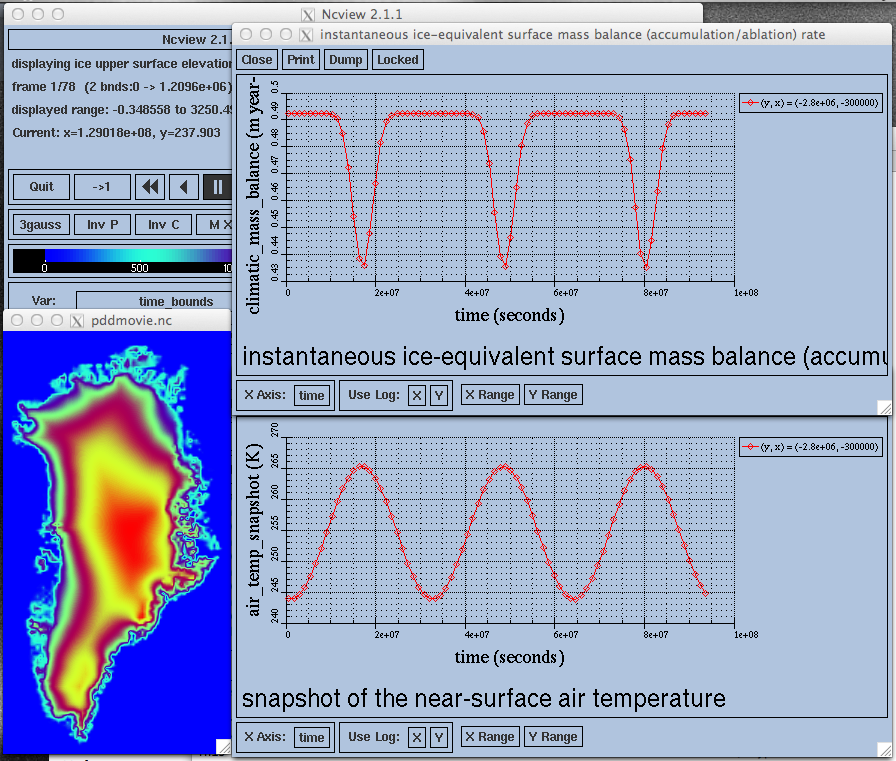
\includegraphics[width=5in]{pdd-movie}
  \caption{Time series of the surface mass balance rate and near-surface air temperature.}
  \label{fig:pddseries}
\end{figure}

\bigskip
We can also test the surface temperature forcing code with the following command.
\begin{verbatim}
$ pismr -i g20km_pre100.nc -surface simple \
          -atmosphere searise_greenland,delta_T \
          -atmosphere_delta_T_file pism_dT.nc \
          -extra_times 100 -ys -125e3 -ye 0 \
          -extra_vars ice_surface_temp \
          -extra_file dT_movie.nc -o_order zyx \
          -test_climate_models -no_mass
\end{verbatim}
%$ - match dollar signs to make emacs happy
The output \texttt{dT_movie.nc} and \texttt{pism_dT.nc} were used to create figure \ref{fig:artm-timeseries}.

This figure shows the GRIP temperature offsets and the time-series of the temperature at the ice surface at a point in southern Greenland (bottom graph), confirming that the temperature offsets are used correctly.

\begin{figure}[ht]
  \centering
  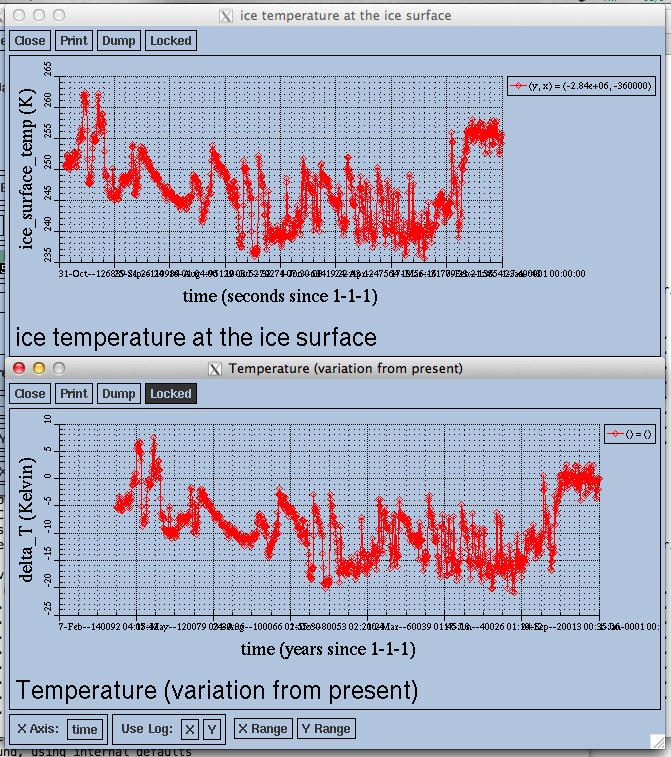
\includegraphics[width=5in]{dT-movie}
  \caption{Time series of the surface temperature compared to GRIP temperature offsets}
  \label{fig:artm-timeseries}
\end{figure}


\clearpage\newpage
\newcommand{\surface}{Surface components (\texttt{-surface}; default: \texttt{given})}
\section{Surface mass and energy process model~components}
\label{sec:surface}

\subsection{The ``invisible'' model}
\label{sec:surface-simple}

\begin{center}
  \begin{tabular}{rp{0.5\linewidth}}
    \toprule
    Command-line option: & \texttt{-surface~simple} \index[options]{SA@\surface!\texttt{simple}}\\
    NetCDF variables: & none \\
    C++ class: & \class{PSSimple}\\
    \bottomrule
  \end{tabular}
\end{center}

This is the simplest ``surface model'' available in PISM, enabled using
\texttt{-surface~simple}. Its job is to re-interpret precipitation as climatic
mass balance, and to re-interprets mean annual near-surface (2m) air
temperature as the temperature of the ice at the depth at which firn processes
cease to change the temperature of the ice. (I.e.~the temperature \emph{below}
the firn.) This implies that there is no melt. Though primitive, this model~component may
be desired in cold environments (e.g.~East Antarctic ice sheet) in which melt
is negligible and heat from firn processes is ignored.

\subsection{Reading top-surface boundary conditions from a file}
\label{sec:surface-given}
\optsection{SA@\surface!\texttt{given}}
\index{One-way coupling to a climate model}

\begin{center}
  \begin{tabular}{rp{0.5\linewidth}}
    \toprule
    Command-line option: & \texttt{-surface~given}
    \index[options]{SA@\surface!\texttt{given}}\\
    NetCDF variables: & \variable{ice_surface_temp}, \\
    &\variable{climatic_mass_balance} [kg/m$^2$/s]\\
    C++ class: & \class{PSGivenClimate}\\
    \bottomrule
  \end{tabular}
\end{center}

\begin{center}
  \bf This is the default choice.
\end{center}

This model~component was created to force PISM with sampled (possibly periodic)
climate data by reading ice upper surface boundary conditions from a file.
These fields are provided directly to the ice dynamics code (see User's
Manual, table~\ref*{manual-tab:ice-dynamics-bc}).

PISM will stop if variables \variable{ice_surface_temp} (ice temperature at the
ice surface but below firn) and \variable{climatic_mass_balance} (top surface
mass flux into the ice) are not present in the input file.

Command-line options:
\begin{itemize}
\item \fileopt{surface_given_file} prescribes an input file
\item \txtopt{surface_given_period}{\emph{years}} makes PISM interpret data in
\texttt{-surface_given_file} as periodic. See section~\ref{sec:periodic-forcing}.
\item \intextoption{surface_given_reference_year} sets the reference model year;
  see section~\ref{sec:periodic-forcing}.
\end{itemize}

A file \texttt{foo.nc} used with \texttt{-surface given -surface_given_file
  foo.nc} should contain several records. If this file contains one record
(i.e. fields corresponding to one time value only), provided forcing data is
interpreted as time-independent. The \variable{time} variable should describe
what model time these records correspond to; see section~\ref{sec:model-time}
for details.

For example, to use monthly records and period of 1 year, create a file (say,
``\texttt{foo.nc}'') with 12 records. The \variable{time} variable may contain
0, 1, 2, 3, \dots, 11 and have the units of ``month'' (you can use other units,
too). Then, run
\begin{verbatim}
$ pismr -surface given -surface_given_file foo.nc -surface_given_period 1
\end{verbatim}
%$ - match dollar signs to make emacs happy

\noindent Notes:
\begin{itemize}
\item This surface model \emph{ignores} the atmosphere model selection made
  using the \texttt{-atmosphere} option.
\item PISM can handle files with virtually any number of records: it will
  read and store in memory at most \config{climate_forcing.buffer_size} records
  at any given time (default: 60, or 5 years' worth of monthly fields).
\item when preparing a file for use with this model, it is best to use the
  \texttt{t,x,y} variable storage order: files using this order can be read in
  faster than ones using the \texttt{t,y,x} order, for reasons explained in the
  User's Manual, section~\ref*{manual-sec:pism-io-performance}.

  To change the storage order in a NetCDF file, use \texttt{ncpdq}:
\begin{verbatim}
$ ncpdq -a t,x,y input.nc output.nc
\end{verbatim}
%$ - match dollar signs to make emacs happy
  will copy data from \texttt{input.nc} into \texttt{output.nc}, changing the
  storage order to \texttt{t,x,y} at the same time.
\end{itemize}

\subsection{Elevation-dependent temperature and mass balance}
\label{sec:surface-elevation}
\optsection{SA@\surface!\texttt{elevation}}

\newcommand{\var}[2]{ {#1}_{\text{#2}} }
\newcommand{\h}[1]{ \var{h}{#1} }
\newcommand{\T}[1]{ \var{T}{#1} }
\newcommand{\m}[1]{ \var{m}{#1} }
\newcommand{\ms}[1]{ \var{m^{*}}{#1} }
\newcommand{\diff}[2]{ \frac{\mathrm{d}#1}{\mathrm{d}#2} }

\begin{center}
  \begin{tabular}{rp{0.5\linewidth}}
    \toprule
    Command-line option: & \texttt{-surface~elevation} \index[options]{SA@\surface!\texttt{elevation}} \\
    NetCDF variables: & none\\
    C++ class: & \class{PSElevation} \\
    \bottomrule
  \end{tabular}
\end{center}

This surface model~component parameterizes the ice surface temperature $T_{h}$ =
\variable{ice_surface_temp} and the mass balance $m$ =
\variable{climatic_mass_balance} as \emph{piecewise-linear} functions of
surface elevation $h$.

The option \txtopt{ice_surface_temp}{\emph{list of 4 numbers}} determines the surface temperature using the 4 parameters $\T{min}$, $\T{max}$, $\h{min}$, $\h{max}$. Let
\begin{equation}
  \diff{T}{h} = (\T{max} - \T{min}) / (\h{max} - \h{min})
\end{equation}
be the temperature gradient. Then
\begin{equation}
  T(x,y) =
  \begin{cases}
    \T{min}, & h(x,y) \le \h{min}, \\
    \T{min} + \diff{T}{h} \, (h(x,y) - \h{min}), & \h{min} < h(x,y) < \h{max}, \\
    \T{max}, & \h{max} \le h(x,y).
  \end{cases}
\end{equation}

The option \txtopt{climatic_mass_balance}{\emph{list of 5 numbers}} determines the surface mass balance using the 5 parameters $\m{min}$, $\m{max}$, $\h{min}$, $\h{ELA}$, $\h{max}$. Let
\begin{equation}
  \diff{\m{abl}}{h} = -\m{min} / (\h{max} - \h{min})
\end{equation}
and
\begin{equation}
\diff{\m{acl}}{h} = \m{max} / (\h{max} - \h{min})
\end{equation}
be the mass balance gradient in the ablation and in the accumulation area, respectively.  Then
\begin{equation}
  m(x,y) =
  \begin{cases}
   \m{min}, & h(x,y) \le \h{min}, \\
   \diff{\m{abl}}{h} \, (h(x,y) - h_{\text{ELA}}), &  \h{min} < h(x,y) < \h{max}, \\
   \diff{\m{acl}}{h} \, (h(x,y) - h_{\text{ELA}}), & \h{min} < h(x,y) < \h{max}, \\
   \m{max}, & \h{max} \le h(x,y).
 \end{cases}
\end{equation}

The option \txtopt{climatic_mass_balance_limits}{\emph{list of 2 numbers}} limits the mass balance below $\h{min}$ to $\ms{min}$ and above $\h{max}$ to $\ms{max}$, thus
\begin{equation}
  m(x,y) =
  \begin{cases}
    m^{*}_{\text{min}}, & h(x,y) \le \h{min}, \\
    \diff{\m{abl}}{h} \, (h(x,y) - h_{\text{ELA}}), & \h{min} < h(x,y) < \h{max}, \\
    \diff{\m{acl}}{h} \, (h(x,y) - h_{\text{ELA}}), & \h{min} < h(x,y) < \h{max}, \\
    m^{*}_{\text{max}}, & \h{max} \le h(x,y).
  \end{cases}
\end{equation}

Note: this surface model \emph{ignores} the atmosphere model selection made using the \texttt{-atmosphere} option.

\subsection{Temperature-index (positive degree-day) scheme}
\label{sec:surface-pdd}
\optsection{SA@\surface!\texttt{pdd}}
\index{temperature-index surface processes model}
\index{positive degree day surface processes model}
\index{PDD (positive degree day model)}

\begin{center}
  \begin{tabular}{rp{0.5\linewidth}}
    \toprule
    Command-line option: & \texttt{-surface~pdd} \index[options]{SA@\surface!\texttt{pdd}} \\
    NetCDF variables: & \variable{air_temp_sd}, \variable{snow_depth} \\
    C++ class: & \class{PSTemperatureIndex}\\
    \bottomrule
  \end{tabular}
\end{center}

\newcommand{\PDD}{\ensuremath{\text{PDD}}}
\newcommand{\Hs}{\ensuremath{H_{\text{snow}}}}
\newcommand{\Ms}{\ensuremath{\text{Melt}_{\text{snow}}}}
\newcommand{\Mi}{\ensuremath{\text{Melt}_{\text{ice}}}}
\begin{figure}
  \centering
  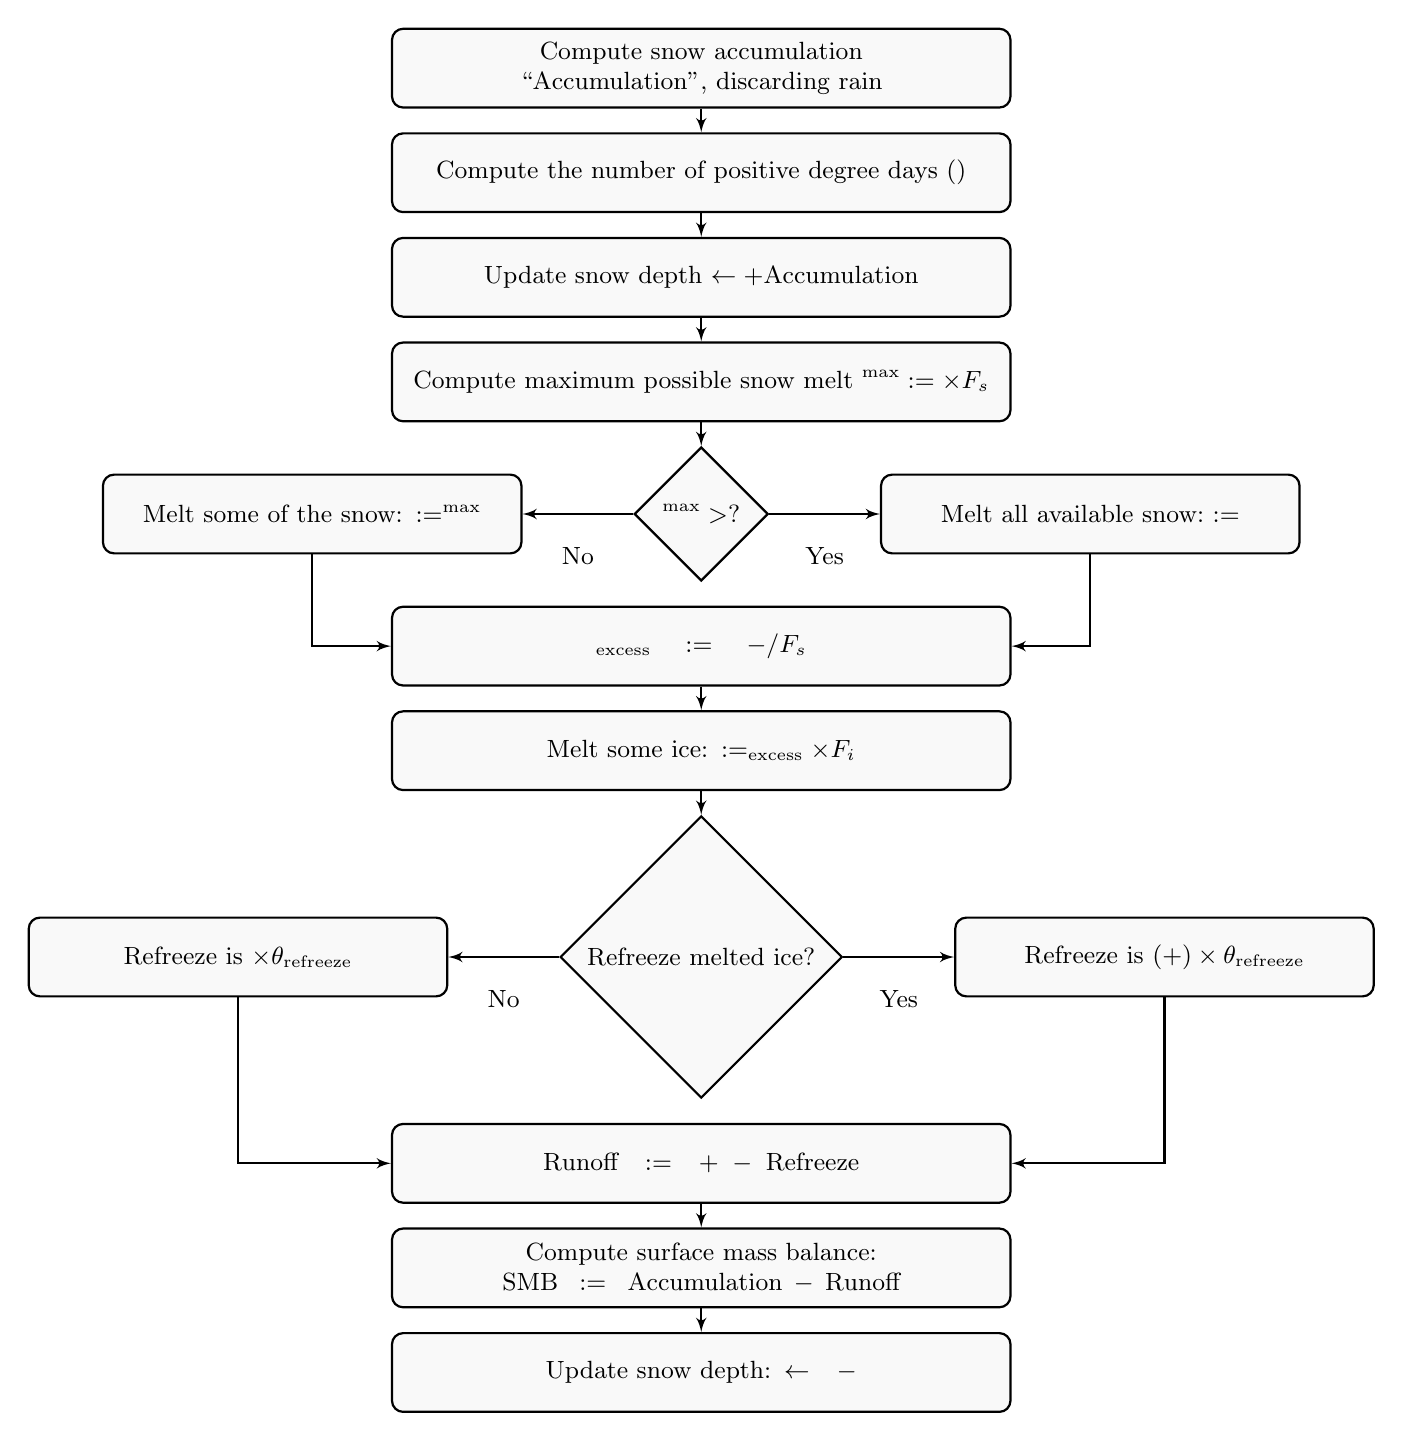
\begin{tikzpicture}[ auto, thick, font=\small, node distance=3mm,
    block/.style={rectangle, rounded corners, draw, fill=gray!5, text width=2in, text centered,
      minimum width=2in, minimum height=1cm},
    big block/.style={block, text width=3in},
    decision/.style={diamond, draw, fill=gray!5},
    line/.style={draw, -latex'},
    start chain=1 going below, every node/.style={on chain},
    every join/.style={-latex'},
    ]

    \node [big block] {Compute snow accumulation \mbox{``Accumulation''}, discarding rain};
    \node [big block, join] {Compute the number of \mbox{positive} degree days (\PDD) };
    \node [big block, join] {Update snow depth \mbox{$\Hs \gets \Hs + \text{Accumulation}$}};
    \node [big block, join] {Compute maximum possible snow melt \mbox{$\Ms^{\text{max}} := \PDD\times F_{s}$}};
    \node (melt all snow) [decision, join] {$\Ms^{\text{max}} > \Hs?$};

    \begin{scope}[start branch=yes, node distance=4em]
      \node (ice melt case) [block, on chain=going right] {\mbox{Melt all available snow:} $\Ms := \Hs$};
    \end{scope}
    \begin{scope}[start branch=no, node distance=4em]
      \node (no ice melt case) [block, on chain=going left] {Melt some of the snow: \mbox{$\Ms := \Ms^{\text{max}}$}};
    \end{scope}

    \node (excess pdds) [big block] {$\PDD_{\text{excess}} := \PDD - \Ms / F_{s}$};
    \node [big block, join] {Melt some ice: \mbox{$\Mi := \PDD_{\text{excess}} \times F_{i}$}};
    \node (refreeze ice) [decision, join] {Refreeze melted ice?};

    \begin{scope}[start branch=yes, node distance=4em]
      \node (refreeze both) [block, on chain=going right] {Refreeze is \mbox{$(\Ms + \Mi) \times \theta_{\text{refreeze}}$}};
    \end{scope}

    \begin{scope}[start branch=no, node distance=4em]
      \node (refreeze snow) [block, on chain=going left] {Refreeze is $\Ms \times \theta_{\text{refreeze}}$};
    \end{scope}

    \node (runoff) [big block] {$\text{Runoff} := \Ms + \Mi - \text{Refreeze}$};
    \node [big block, join] {Compute surface mass balance: $\text{SMB} := \text{Accumulation} - \text{Runoff}$};
    \node [big block, join] {Update snow depth: $\Hs \gets \Hs - \Ms$};
    % special edges:
    \path[line] (melt all snow) -- node {Yes} (ice melt case);
    \path[line] (melt all snow) -- node {No}  (no ice melt case);
    \path[line] (ice melt case) |- (excess pdds);
    \path[line] (no ice melt case) |- (excess pdds);
    \path[line] (refreeze ice) -- node {Yes} (refreeze both);
    \path[line] (refreeze ice) -- node {No}  (refreeze snow);
    \path[line] (refreeze both) |- (runoff);
    \path[line] (refreeze snow) |- (runoff);
  \end{tikzpicture}
  \caption{PISM's positive degree day model. $F_s$ and $F_i$ are PDD
    factors for snow and ice, respectively; $\theta_{\text{refreeze}}$
    is the refreeze fraction.}
  \label{fig:pdd-model}
\end{figure}

The default PDD model used by PISM, turned on by option
\texttt{-surface pdd}, is based on~\cite{CalovGreve05} and
EISMINT-Greenland intercomparison (see~\cite{RitzEISMINT}).

Our model computes the solid (snow) precipitation rate using the air
temperature threshold with a linear transition. All precipitation
during periods with air temperatures above
\config{air_temp_all_precip_as_rain} (default of $2^\circ C$) is
interpreted as rain; all precipitation during periods with air
temperatures below \config{air_temp_all_precip_as_snow} (default of
$0^\circ C$) is interpreted as snow.

For long-term simulations, a PDD model generally uses an idealized
seasonal temperature cycle. ``White noise'' is added to this cycle to simulate
additional daily variability associated to the vagaries of weather. This
additional random variation is quite significant, as the seasonal cycle may
never reach the melting point but that point may be reached with some
probability, in the presence of the daily variability, and thus melt may occur.
Concretely, a normally-distributed, mean zero random temperature increment is
added to the seasonal cycle. There is no assumed spatial correlation of daily
variability. The standard deviation of the daily variability is controlled by
command-line options:

\begin{itemize}
\item \fileopt{pdd_sd_file}, which prescribes an input file.
\item \txtopt{pdd_sd_period}{\emph{years}}, which interprets its data
  as periodic; see section~\ref{sec:periodic-forcing}.
\item \intextoption{pdd_sd_reference_year}, which sets the reference model year;
  see section~\ref{sec:periodic-forcing}.
\end{itemize}

A file \texttt{foo.nc} used with \texttt{-surface pdd -pdd_sd_file foo.nc}
should contain standard deviation of near-surface air temperature in variable
\variable{air_temp_sd}, and the corresponding time coordinate in variable
\variable{time}. If \texttt{-pdd_sd_file} is not set, PISM uses a constant
value for standard deviation, which is set by the \texttt{pdd_std_dev}
configuration parameter. The default value is $5.0$ degrees \cite{RitzEISMINT}.
However, this approach is not recommended as it induces significant errors in
modeled surface mass balance in both ice-covered and ice-free regions
\cite{RogozhinaRau2014, Seguinot2013}.

Over ice-covered grid cells, daily variability can also be parameterized as a linear function of near-surface air temperature $\sigma = a*T + b$ using the \config{pdd_std_dev_use_param} configuration flag, and the corresponding parameters \config{pdd_std_dev_param_a} and \config{pdd_std_dev_param_b}. This parametrization replaces prescribed standard deviation values over glacierized grid cells as defined by the \variable{mask} variable (see \config{geometry.ice_free_thickness_standard}). Default values for the slope $a$ and intercept $b$ were derived from the ERA-40 reanalysis over the Greenland ice sheet \cite{SeguinotRogozhina2014}.

The number of positive degree days is computed as the magnitude of the
temperature excursion above $0\!\phantom{|}^\circ \text{C}$ multiplied by the
duration (in days) when it is above zero.

In PISM there are two methods for computing the number of positive degree days.
The first computes only the expected value, by the method described in
\cite{CalovGreve05}. This is the default when a PDD is chosen (i.e.~option
\texttt{-surface~pdd}). The second is a Monte Carlo simulation of the white
noise itself, chosen by adding the option \intextoption{pdd_rand}. This Monte
Carlo simulation adds the same daily variation at every point, though the
seasonal cycle is (generally) location dependent. If repeatable randomness is
desired use \intextoption{pdd_rand_repeatable} instead of \texttt{-pdd_rand}.

By default, the computation summarized in Figure \ref{fig:pdd-model}
is performed every week. (This frequency is controlled by the
\config{pdd_max_evals_per_year} parameter.) To compute mass balance
during each week-long time-step, PISM keeps track of the current snow
depth (using units of ice-equivalent thickness). This is necessary to
determine if melt should be computed using the degree day factor for
snow (\config{pdd_factor_snow}) or the corresponding factor for ice
(\config{pdd_factor_ice}).

A fraction of the melt controlled by the configuration parameter
\config{pdd_refreeze} ($\theta_{\text{refreeze}}$ in Figure
\ref{fig:pdd-model}, default: $0.6$) refreezes. The user can select
whether melted ice should be allowed to refreeze using the
\config{pdd_refreeze_ice_melt} configuration flag.

Since PISM does not have a principled firn model, the snow depth is
set to zero at the beginning of the balance year. See
\config{pdd_balance_year_start_day}. Default is $274$, corresponding
to October 1$^{\text{st}}$.

Our PDD implementation is meant to be used with an atmosphere model
implementing a cosine yearly cycle such as \texttt{searise_greenland} (section
\ref{sec:atmosphere-searise-greenland}), but it is not restricted to
parameterizations like these.

This code also implements latitude- and mean July temperature dependent ice and snow
factors using formulas (6) and (7) in~\cite{Faustoetal2009}; set
\intextoption{pdd_fausto} to enable. The default standard deviation of the
daily variability (\intextoption{pdd_std_dev} option) is 2.53 degrees under the
\intextoption{pdd_fausto} option~\cite{Faustoetal2009}. See also configuration
parameters with the \texttt{pdd_fausto} prefix.

Note that when used with periodic climate data (air temperature and
precipitation) that is read from a file (see section
\ref{sec:atmosphere-given}), use of \texttt{-timestep_hit_multiplies
  X} is recommended. (Here \texttt{X} is the length of the climate
data period in years.)

\subsection{PIK}
\label{sec:surface-pik}

\begin{center}
  \begin{tabular}{rp{0.5\linewidth}}
    \toprule
    Command-line option: & \texttt{-surface~pik} \index[options]{SA@\surface!\texttt{pik}} \\
    NetCDF variables: & \variable{climatic_mass_balance} [kg/m$^2$/s],\\
    &\variable{lat} (latitude), [degrees north]\\
    C++ class: & \class{PSConstantPIK}\\
    \bottomrule
  \end{tabular}
\end{center}

This surface model~component implements the setup used in~\cite{Martinetal2011}. The
\variable{climatic_mass_balance} is read from an input (\texttt{-i}) file; the ice surface temperature is computed as a function of
latitude (variable \variable{lat}) and surface elevation (dynamically updated
by PISM). See equation~(1) in~\cite{Martinetal2011}.

\newcommand{\surfacemods}{Surface modifiers}
\subsection{Modifier: Scalar temperature offsets}
\label{sec:surface-delta-T}
\optsection{SB@\surfacemods!\texttt{delta_T}}

\begin{center}
  \begin{tabular}{rp{0.5\linewidth}}
    \toprule
    Command-line option: & \texttt{-surface~...,delta_T} \index[options]{SB@\surfacemods!\texttt{delta_T}} \\
    NetCDF variables: & \variable{delta_T} \\
    C++ class: & \class{PS_delta_T}\\
    \bottomrule
  \end{tabular}
\end{center}

Command-line options:
\begin{itemize}
\item \fileopt{surface_delta_T_file} sets the name of the
file PISM will read \variable{delta_T} from.
\item \txtopt{surface_delta_T_period}{\emph{years}} sets the period of the
  forcing data (section~\ref{sec:periodic-forcing})
\item \intextoption{surface_delta_T_reference_year} sets the reference year (section~\ref{sec:periodic-forcing}).
\end{itemize}

The time-dependent scalar offsets \variable{delta_T} are added to
\variable{ice_surface_temp} computed by a surface model.

Please make sure that \variable{delta_T} has the units of
``\texttt{Kelvin}''.

This modifier is identical to the corresponding atmosphere modifier, but
applies offsets at a different stage in the computation of top-surface boundary
conditions needed by the ice dynamics core.

\subsection{Modifier: Lapse rate corrections}
\label{sec:surface-lapse-rate}
\optsection{SB@\surfacemods!\texttt{lapse_rate}}

\begin{center}
  \begin{tabular}{rp{0.5\linewidth}}
    \toprule
    Command-line option: & \texttt{-surface~...,lapse_rate} \index[options]{SB@\surfacemods!\texttt{lapse_rate}} \\
    NetCDF variables: & \variable{surface_altitude} (CF standard name), \\
    C++ class: & \class{PSLapseRates}\\
    \bottomrule
  \end{tabular}
\end{center}

The \texttt{lapse_rate} modifier allows correcting ice-surface temperature and
surface mass balance using elevation lapse rates. It uses the following
options.

\begin{itemize}
\item \intextoption{temp_lapse_rate} gives the temperature lapse rate, in
  $K/km$. Note that we use the following definition of the temperature lapse
  rate:
  \begin{displaymath}
    \gamma = -\frac{dT}{dz}.
  \end{displaymath}
\item \intextoption{smb_lapse_rate} gives the surface mass balance lapse rate,
  in $m/year/km$. Here, $\gamma=-\frac{dM}{dz}$.
\item \fileopt{surface_lapse_rate_file} specifies the file containing the reference
  surface elevation field (standard name: \variable{surface_altitude}). This file
  can contain several surface elevation records to use lapse rate corrections
  relative to time-dependent surface. If one record is provided, the reference
  surface elevation is assumed to be time-independent.
\item \intextoption{surface_lapse_rate_period} gives the period, in model years, to
  use when interpreting data in the file given with
  \texttt{-surface_given_file},
\item \intextoption{surface_lapse_rate_reference_year} takes the time $T$ in model
  years. The record for $t$ years in \texttt{-surface_given_file} is
  interpreted as corresponding to $t$ years since $T$.
\end{itemize}

\subsection{Modifier: Surface mass flux adjustment}
\label{sec:smb-adjustment}
\optsection{SB@\surfacemods!\texttt{forcing}}

\begin{center}
  \begin{tabular}{rp{0.5\linewidth}}
    \toprule
    Command-line option: & \texttt{-surface~...,forcing} \index[options]{SB@\surfacemods!\texttt{forcing}} \\
    NetCDF variables: & \variable{thk} (ice thickness), \variable{ftt_mask} (mask of zeros and ones; 1 where surface mass flux is adjusted and 0 elsewhere) \\
    C++ class: & \class{PSForceThickness}\\
    \bottomrule
  \end{tabular}
\end{center}

The \texttt{forcing} modifier implements a surface mass balance adjustment
mechanism which forces the thickness of grounded ice to a target thickness distribution at the
end of the run. The idea behind this mechanism is that spinup of ice sheet
models frequently requires the surface elevation to come close to measured
values at the end of a run. A simpler alternative to accomplish this, namely
option \texttt{-no_mass}, represents an unmodeled, frequently large,
violation of the mass continuity equation.

In more detail, let $H_{\text{tar}}$ be the target thickness. Let $H$ be the
time-dependent model thickness. The surface model~component described
here produces the term $M$ in the mass continuity equation:
\begin{displaymath}
\frac{\partial H}{\partial t} = M - S - \nabla\cdot \mathbf{q}.
\end{displaymath}
(Other details of this equation do not concern us here.) The
\texttt{forcing} modifier causes $M$ to be adjusted by a multiple of
the difference between the target thickness and the current thickness,
\begin{displaymath}
\Delta M = \alpha (H_{\text{tar}} - H)
\end{displaymath}
where $\alpha>0$. We are adding mass ($\Delta M>0$) where $H_{\text{tar}} > H$
and ablating where $H_{\text{tar}} < H$.

Option \fileopt{force_to_thickness_file} identifies the file containing the target ice
thickness field \texttt{thk} and the mask \texttt{ftt_mask}. A basic run modifying surface model \texttt{given} would look like
\begin{verbatim}
$ pismr -i foo.nc -surface given,forcing -force_to_thickness_file bar.nc
\end{verbatim}
%$ - match dollar signs to make emacs happy

In this case \texttt{foo.nc} contains fields \variable{climatic_mass_balance} and \variable{ice_surface_temp}, as normal for \texttt{-surface~given}, and \texttt{bar.nc} contains fields
\variable{thk} which will serve as the target thickness and \variable{ftt_mask} which defines the map plane area where this adjustment is applied. Option
\intextoption{force_to_thickness_alpha} adjusts the value of $\alpha$, which has a
default value specified in the \emph{Source Code Browser}
\url{\PISMBROWSERURL}.

In addition to this one can specify a multiplicative factor $C$ used in areas where the target thickness field has less than \intextoption{force_to_thickness_ice_free_thickness_threshold} meters of ice; $\alpha_{\text{ice free}} = C \times \alpha$. Use the \intextoption{force_to_thickness_ice_free_alpha_factor} option to set $C$.

\subsection{Modifier: Anomalies}
\label{sec:surface-anomaly}
\optsection{SB@\surfacemods!\texttt{anomaly}}

\begin{center}
  \begin{tabular}{rp{0.5\linewidth}}
    \toprule
    Command-line option: & \texttt{-surface~...,anomaly} \index[options]{SB@\surfacemods!\texttt{anomaly}} \\
    NetCDF variables: & \variable{ice_surface_temp_anomaly}, \\
    &\variable{climatic_mass_balance_anomaly} \mbox{[kg/m$^2$/s]}\\
    C++ class: & \class{PSAnomaly}\\
    \bottomrule
  \end{tabular}
\end{center}

This modifier implements a spatially-variable version of \texttt{-surface
  ...,delta_T} which also applies time-dependent climatic mass balance anomalies.

It takes the following options:
\begin{itemize}
\item \fileopt{surface_anomaly_file} specifies a file containing variables
  \variable{ice_surface_temp_anomaly} and
  \variable{climatic_mass_balance_anomaly}.
\item \txtopt{surface_anomaly_period}{years} specifies the period of the
  forcing data, in model years; section~\ref{sec:periodic-forcing}
\item \intextoption{surface_anomaly_reference_year} specifies the reference
  year; section~\ref{sec:periodic-forcing}.
\end{itemize}

See also to \texttt{-atmosphere~...,anomaly}
(section~\ref{sec:atmosphere-anomaly}), which is similar, but applies anomalies
at the atmosphere level.

\subsection{Modifier: Caching}
\label{sec:surface-cache}
\optsection{SB@\surfacemods!\texttt{cache}}

\begin{center}
  \begin{tabular}{rp{0.5\linewidth}}
    \toprule
    Command-line option: & \texttt{-surface~...,cache} \index[options]{SB@\surfacemods!\texttt{cache}} \\
    C++ class: & \class{PSCache}\\
    \bottomrule
  \end{tabular}
\end{center}

This modifier skips surface model updates, so that a surface model is
called no more than every \texttt{-surface_cache_update_interval}
years. A time-step of $1$ year is used every time a surface model is
updated.

This is useful in cases when inter-annual climate variability is
important, but one year differs little from the next. (Coarse-grid
paleo-climate runs, for example.)

It takes the following options:
\begin{itemize}
\item \txtopt{surface_cache_update_interval}{\emph{years}} Specifies the
  minimum interval between updates. PISM may take longer time-steps if
  the adaptive scheme allows it, though.
\end{itemize}

See also section \ref{sec:ocean-cache}.

\clearpage\newpage

\newcommand{\atmosphere}{Atmosphere components (\texttt{-atmosphere};
  default: \texttt{given})}
\section{Atmosphere model~components}
\label{sec:atmosphere}

\subsection{Reading atmosphere boundary conditions from a file}
\label{sec:atmosphere-given}
\optsection{\atmosphere!\texttt{given}}
\index{One-way coupling to a climate model}

\begin{center}
  \begin{tabular}{rp{0.5\linewidth}}
    \toprule
    Command-line option: & \texttt{-atmosphere~given} \index[options]{\atmosphere!\texttt{given}} \\
    NetCDF variables: & \variable{air_temp}, \\
    &\variable{precipitation} [m/s ice equivalent]\\
    C++ class: & \class{PAGivenClimate}\\
    \bottomrule
  \end{tabular}
\end{center}

\begin{center}
  \bf This is the default choice.
\end{center}

Command-line options:
\begin{itemize}
\item \fileopt{atmosphere_given_file} prescribes an input file
\item \txtopt{atmosphere_given_period}{\emph{years}} makes PISM interpret data in
\texttt{-atmosphere_given_file} as periodic. See section~\ref{sec:periodic-forcing}.
\item \intextoption{atmosphere_given_reference_year} sets the reference model year;
  see section~\ref{sec:periodic-forcing}.
\end{itemize}

A file \texttt{foo.nc} used with \texttt{-atmosphere given -atmosphere_given_file foo.nc} should contain several records; the \variable{time} variable should describe what model time these records correspond to.

This model~component was created to force PISM with sampled (possibly periodic) climate data, e.g. using monthly records of \variable{air_temp} and \variable{precipitation}.

It can also used to drive a temperature-index (PDD) climatic mass balance
computation (section~\ref{sec:surface-pdd}).

See also section~\ref{sec:surface-given}, which describes a similar surface
model~component (\texttt{-surface~given}).

\subsection{Cosine yearly cycle}
\label{sec:cosine-yearly-cycle}
\optsection{\atmosphere!\texttt{yearly_cycle}}

\begin{center}
  \begin{tabular}{rp{0.5\linewidth}}
    \toprule
    Command-line option: & \texttt{-atmosphere~yearly_cycle}
    \index[options]{\atmosphere!\texttt{yearly_cycle}} \\
    NetCDF variables: & \variable{air_temp_mean_annual},\\
    &\variable{air_temp_mean_july},\\
    &\variable{precipitation} \mbox{[m/s ice equivalent]}\\
    &\variable{amplitude_scaling} \\
    C++ class: & \class{PACosineYearlyCycle}\\
    \bottomrule
  \end{tabular}
\end{center}

This atmosphere model~component computes the near-surface air temperature using the following formula:
\begin{displaymath}
  T(\mathrm{time}) = T_{\text{mean annual}} + A(\mathrm{time})\cdot(T_{\text{mean July}} - T_{\text{mean annual}}) \cdot \cos(2\pi t),
\end{displaymath}
where $t$ is the year fraction ``since last July''; the summer peak of the cycle is on \config{atmosphere.fausto_air_temp.summer_peak_day}, which is set to day $196$ by default (approximately July 15).

Here $T_{\text{mean annual}}$ (variable \variable{air_temp_mean_annual}) and $T_{\text{mean July}}$ (variable \variable{air_temp_mean_july}) are read from a file selected using the \intextoption{atmosphere_yearly_cycle_file} command-line option. A time-independent precipitation field (variable \variable{precipitation}) is read from the same file.

Optionally a time-dependent scalar amplitude scaling $A(t)$ can be used. Specify a file to read it from using the  \intextoption{atmosphere_yearly_cycle_scaling_file} command-line option. Without this option $A(\mathrm{time}) \equiv 1$.

\subsection{SeaRISE-Greenland}
\label{sec:atmosphere-searise-greenland}
\optsection{\atmosphere!\texttt{searise_greenland}}

\begin{center}
  \begin{tabular}{rp{0.5\linewidth}}
    \toprule
    Command-line option: & \texttt{-atmosphere~searise_greenland} \index[options]{\atmosphere!\texttt{searise_greenland}} \\
    NetCDF variables: & \variable{lon}, \variable{lat},
    \variable{precipitation} \mbox{[m/s ice equivalent]}\\
    C++ class: & \class{PASeariseGreenland}\\
    \bottomrule
  \end{tabular}
\end{center}

This atmosphere model~component implements a longitude, latitude, and elevation dependent near-surface air temperature parameterization and a cosine yearly cycle described in~\cite{Faustoetal2009} and uses a constant in time ice-equivalent precipitation field (in units of thickness per time, variable \variable{precipitation}) that is read from an input (\texttt{-i}) file. To read time-independent precipitation from a different file, use the option \intextoption{atmosphere_searise_greenland_file}.

The air temperature parameterization is controlled by configuration parameters with the \texttt{snow_temp_fausto} prefix.

See also the \texttt{-atmosphere ...,paleo_precip} modifier, section
\ref{sec:atmosphere-paleo-precip}, for an implementation of the
SeaRISE-Greenland formula for paleo-precipitation correction from
present; a 7.3\% change of precipitation rate for every one degree
Celsius of temperature change~\cite{Huybrechts02}.

\subsection{PIK}
\label{sec:atmosphere-pik}

\begin{center}
  \begin{tabular}{rp{0.5\linewidth}}
    \toprule
    Command-line option: & \texttt{-atmosphere~pik}
    \index[options]{\atmosphere!\texttt{pik}}  \\
    NetCDF variables: & \variable{lat}, \variable{precipitation} \\
    C++ class: & \class{PAConstantPIK}\\
    \bottomrule
  \end{tabular}
\end{center}

This model~component reads a time-independent precipitation field from an input
(\texttt{-i}) file and computes near-surface air
temperature using a latitude and surface elevation-dependent formula.

The parameterization is the same as in the \texttt{-surface pik} model,
section~\ref{sec:surface-pik}.

\subsection{One weather station}
\label{sec:atmosphere-one-station}

\begin{center}
  \begin{tabular}{rp{0.5\linewidth}}
    \toprule
    \index[options]{\atmosphere!\texttt{one_station}}
    \index[options]{\atmosphere!\texttt{one_station}!\texttt{-atmosphere_one_station_file}}
    Command-line options: & \texttt{-atmosphere~one_station},\\
                          & \texttt{-atmosphere_one_station_file}\\
    NetCDF variables:     & \variable{air_temp} [Kelvin],\\
                          & \variable{precipitation} [m / s ice equivalent]\\
    C++ class:            & \class{PAWeatherStation}\\
    \bottomrule
  \end{tabular}
\end{center}

This model~component reads scalar time-series of the near-surface air
temperature and precipitation from a file specified using the
\mbox{\texttt{-atmosphere_one_station_file}} option and uses them at \emph{all}
grid points in the domain. In other words, resulting climate fields
are constant in space but not necessarily in time.

The \texttt{-atmosphere~one_station} model should be used with a
modifier such as \texttt{lapse_rate} (see section
\ref{sec:atmosphere-lapse-rates}) to create spatial variablitity.

\newcommand{\atmospheremods}{Atmosphere modifiers (\texttt{-atmosphere})}
\subsection{Modifier: Scalar temperature offsets}
\label{sec:atmosphere-delta-temp}
\optsection{\atmospheremods!\texttt{delta_T}}

\begin{center}
  \begin{tabular}{rp{0.5\linewidth}}
    \toprule
    Command-line option: & \texttt{-atmosphere~...,delta_T} \index[options]{\atmospheremods!\texttt{delta_T}} \\
    NetCDF variables: & \variable{delta_T} \\
    C++ class: & \class{PA_delta_T}\\
    \bottomrule
  \end{tabular}
\end{center}

This modifier applies scalar time-dependent air temperature offsets to the
output of an atmosphere model. It takes the following command-line options.
\begin{itemize}
\item \fileopt{atmosphere_delta_T_file} sets the name of the
file PISM will read \variable{delta_T} from.
\item \txtopt{atmosphere_delta_T_period}{\emph{years}} sets the period of the
  forcing data (section~\ref{sec:periodic-forcing}).
\item \intextoption{atmosphere_delta_T_reference_year} sets the reference year (section~\ref{sec:periodic-forcing}).
\end{itemize}

Please make sure that \variable{delta_T} has the units of
``\texttt{Kelvin}''.

\subsection{Modifier: Scalar precipitation offsets}
\label{sec:atmosphere-delta-precip}
\optsection{\atmospheremods!\texttt{delta_P}}

\begin{center}
  \begin{tabular}{rp{0.5\linewidth}}
    \toprule
    Command-line option: & \texttt{-atmosphere~...,delta_P} \index[options]{\atmospheremods!\texttt{delta_P}} \\
    NetCDF variables: & \variable{delta_P} \mbox{[m/s ice equivalent]}\\
    C++ class: & \class{PA_delta_P}\\
    \bottomrule
  \end{tabular}
\end{center}

This modifier applies scalar time-dependent precipitation  offsets to the
output of an atmosphere model. It takes the following command-line options.
\begin{itemize}
\item \fileopt{atmosphere_delta_P_file} sets the name of the
file PISM will read \variable{delta_P} from.
\item \txtopt{atmosphere_delta_P_period}{\emph{years}} sets the period of the
  forcing data (section~\ref{sec:periodic-forcing}).
\item \intextoption{atmosphere_delta_P_reference_year} sets the reference year (section~\ref{sec:periodic-forcing}).
\end{itemize}

\subsection{Modifier: Scalar precipitation scaling}
\label{sec:atmosphere-frac-precip}
\optsection{\atmospheremods!\texttt{frac_P}}

\begin{center}
  \begin{tabular}{rp{0.5\linewidth}}
    \toprule
    Command-line option: & \texttt{-atmosphere~...,frac_P} \index[options]{\atmospheremods!\texttt{frac_P}} \\
    NetCDF variables: & \variable{frac_P} \mbox{[no unit]}\\
    C++ class: & \class{PA_frac_P}\\
    \bottomrule
  \end{tabular}
\end{center}

This modifier scales precipitation output of an atmosphere model using a scalar
time-dependent precipitation fraction, with a value of one corresponding to no
change in precipitation. It takes the following command-line options:

\begin{itemize}
  \item \fileopt{atmosphere_frac_P_file}
    sets the name of the file PISM will read \variable{frac_P} from.
  \item \txtopt{atmosphere_frac_P_period}{\emph{years}}
    sets the period of the forcing data (section~\ref{sec:periodic-forcing}).
  \item \intextoption{atmosphere_frac_P_reference_year}
    sets the reference year (section~\ref{sec:periodic-forcing}).
\end{itemize}

\subsection{Modifier: Paleo-precipitation correction using scalar temperature offsets}
\label{sec:atmosphere-paleo-precip}
\optsection{\atmospheremods!\texttt{paleo_precip}}

\begin{center}
  \begin{tabular}{rp{0.5\linewidth}}
    \toprule
    Command-line option: & \texttt{-atmosphere~...,paleo_precip} \index[options]{\atmospheremods!\texttt{paleo_precip}} \\
    NetCDF variables: & \variable{delta_T} \mbox{[degrees Kelvin]}\\
    C++ class: & \class{PA_paleo_precip}\\
    \bottomrule
  \end{tabular}
\end{center}

This modifier implements the SeaRISE-Greenland formula for
paleo-precipitation correction from present; a 7.3\% change of
precipitation rate for every one degree Celsius of air temperature
change~\cite{Huybrechts02}. See
\url{http://websrv.cs.umt.edu/isis/index.php/Model_Initialization#Greenland}
for details. The input file should contain air temperature offsets in
the format used by \texttt{-atmosphere ...,delta_T} modifier, see
section \ref{sec:atmosphere-delta-temp}.

It takes the following command-line options.
\begin{itemize}
\item \fileopt{atmosphere_paleo_precip_file} sets the name of the
file PISM will read \variable{delta_T} from.
\item \txtopt{atmosphere_paleo_precip_period}{\emph{years}} sets the period of the
  forcing data (section~\ref{sec:periodic-forcing}).
\item \intextoption{atmosphere_paleo_precip_reference_year} sets the reference year (section~\ref{sec:periodic-forcing}).
\end{itemize}


\subsection{Modifier: Lapse rate corrections}
\label{sec:atmosphere-lapse-rates}
\optsection{\atmospheremods!\texttt{lapse_rate}}

\begin{center}
  \begin{tabular}{rp{0.5\linewidth}}
    \toprule
    Command-line option: & \texttt{-atmosphere~...,lapse_rate} \index[options]{\atmospheremods!\texttt{lapse_rate}} \\
    NetCDF variables: & \variable{surface_altitude} (CF standard name) \\
    C++ class: & \class{PALapseRates}\\
    \bottomrule
  \end{tabular}
\end{center}

The \texttt{lapse_rate} modifier allows for correcting air temperature and
precipitation using elevation lapse rates. It uses the following options.

\begin{itemize}
\item \intextoption{temp_lapse_rate} gives the temperature lapse rate, in
  $K/km$. Note that we use the following definition of the temperature lapse
  rate:
  \begin{displaymath}
    \gamma = -\frac{dT}{dz}.
  \end{displaymath}
\item \intextoption{precip_lapse_rate} gives the precipitation lapse rate, in
  $m/year/km$. Here $\gamma = -\frac{dM}{dz}$.
\item \fileopt{atmosphere_lapse_rate_file} specifies a file containing the
  reference surface elevation field (standard name:
  \variable{surface_altitude}). This file may contain several surface elevation
  records to use lapse rate corrections relative to a time-dependent surface.
  If one record is provided, the reference surface elevation is assumed to be
  time-independent.
\item \intextoption{atmosphere_lapse_rate_period} gives the period, in model
  years; see section~\ref{sec:periodic-forcing}.
\item \intextoption{atmosphere_lapse_rate_reference_year} specifies the reference date; see section~\ref{sec:periodic-forcing}.
\end{itemize}

\subsection{Modifier: Anomalies}
\label{sec:atmosphere-anomaly}
\optsection{\atmospheremods!\texttt{anomaly}}

\begin{center}
  \begin{tabular}{rp{0.5\linewidth}}
    \toprule
    Command-line option: & \texttt{-atmosphere~...,anomaly} \index[options]{\atmospheremods!\texttt{anomaly}} \\
    NetCDF variables: & \variable{air_temp_anomaly}, \\
    &\variable{precipitation_anomaly} [m/s ice equivalent]\\
    C++ class: & \class{PAAnomaly}\\
    \bottomrule
  \end{tabular}
\end{center}

This modifier implements a spatially-variable version of
\texttt{-atmosphere~...,delta_T,delta_P}.

It takes the following options:
\begin{itemize}
\item \fileopt{atmosphere_anomaly_file} specifies a file containing variables
  \variable{air_temp_anomaly} and
  \variable{precipitation_anomaly}.
\item \txtopt{atmosphere_anomaly_period}{years} specifies the period of the
  forcing data, in model years; section~\ref{sec:periodic-forcing}.
\item \intextoption{atmosphere_anomaly_reference_year} specifies the reference
  year; section~\ref{sec:periodic-forcing}.
\end{itemize}

See also to \texttt{-surface~...,anomaly}
(section~\ref{sec:surface-anomaly}), which is similar, but applies anomalies
at the surface level.


\clearpage\newpage

\newcommand{\ocean}{Ocean components (\texttt{-ocean}; default: \texttt{constant})}
\section{Ocean model~components}
\label{sec:pism-ocean-models}

PISM Ocean model~components provide sub-shelf ice temperature (\variable{shelfbtemp}) and sub-shelf mass flux (\variable{shelfbmassflux}) to the ice dynamics core.

The sub-shelf ice temperature is used as a Dirichlet boundary condition in the energy conservation code. The sub-shelf mass flux is used as a source in the mass-continuity (transport) equation. Positive flux corresponds to ice loss; in other words, this sub-shelf mass flux is a ``melt rate''.

\subsection{Constant in time and space}
\label{sec:ocean-constant}
\optsection{OA@\ocean!\texttt{constant}}

\begin{center}
  \begin{tabular}{rp{0.5\linewidth}}
    \toprule
    Command-line option: & \texttt{-ocean~constant} \index[options]{OA@\ocean!\texttt{constant}} \\
    NetCDF variables: & none \\
    C++ class: & \class{POConstant}\\
    \bottomrule
  \end{tabular}
\end{center}

\begin{center}
  \bf This is the default choice.
\end{center}

This ocean model~component implements boundary conditions at the ice/ocean interface that are constant \textbf{both} in space and time.

The sub-shelf ice temperature is set to pressure melting and the sub-shelf melt rate is assumed to be proportional to the heat flux from the ocean into the ice (configuration parameter\\ \texttt{ocean_sub_shelf_heat_flux_into_ice}).

Alternatively, the sub-shelf melt rate in meters per year can be set using the \intextoption{shelf_base_melt_rate} command-line option.

\subsection{Reading forcing data from a file}
\label{sec:ocean-given}
\optsection{OA@\ocean!\texttt{given}}

\begin{center}
  \begin{tabular}{rp{0.5\linewidth}}
    \toprule
    Command-line option: & \texttt{-ocean~given}
    \index[options]{OA@\ocean!\texttt{given}} \\
    NetCDF variables: & \variable{shelfbtemp}  \mbox{[degrees Kelvin]}, \variable{shelfbmassflux}  \mbox{[kg m-2 s-1]}\\
    C++ class: & \class{POGivenClimate}\\
    \bottomrule
  \end{tabular}
\end{center}

This ocean model~component reads sub-shelf ice temperature \variable{shelfbtemp} and the sub-shelf mass flux \variable{shelfbmassflux} from a file. It takes the following command-line options.
\begin{itemize}
\item \fileopt{ocean_given_file}: sets the name of the file to read forcing data from. The file may contain several records. If only one record is provided it is interpreted as time-independent.
\item \intextoption{ocean_given_reference_year} specifies the reference date; see section~\ref{sec:periodic-forcing}.
\item \intextoption{ocean_given_period} specifies the length of the period of the forcing data, in model years; see section~\ref{sec:periodic-forcing}.
\end{itemize}

Variables \variable{shelfbtemp} and \variable{shelfbmassflux} may be
time-dependent. (The \texttt{-ocean given} component is very similar to
\texttt{-surface~given} and \texttt{-atmosphere~given}.)

\subsection{PIK}
\label{sec:ocean-pik}
\optsection{OA@\ocean!\texttt{pik}}

\begin{center}
  \begin{tabular}{rp{0.5\linewidth}}
    \toprule
    Command-line option: & \texttt{-ocean~pik} \index[options]{OA@\ocean!\texttt{pik}} \\
    NetCDF variables: & none \\
    C++ class: & \class{POConstantPIK}\\
    \bottomrule
  \end{tabular}
\end{center}

This ocean model~component implements the ocean forcing setup used in~\cite{Martinetal2011}. The sub-shelf ice temperature is set to pressure-melting; the sub-shelf mass flux computation follows~\cite{BeckmannGoosse2003}.

It takes one command-line option:
\begin{itemize}
\item \intextoption{meltfactor_pik}: a melt factor $F_{\mathrm{melt}}$ in sub-shelf-melting parameterization, see equation~(5) in~\cite{Martinetal2011}.
\end{itemize}

\subsection{Basal melt rate and temperature from thermodynamics in boundary layer}
\label{sec:ocean-th}
\optsection{OA@\ocean!\texttt{th}}

\begin{center}
  \begin{tabular}{rp{0.5\linewidth}}
    \toprule
    Command-line option: & \texttt{-ocean~th} \index[options]{OA@\ocean!\texttt{th}} \\
    NetCDF variables: & \variable{theta_ocean} (absolute potential ocean temperature), [Kelvin], \variable{salinity_ocean} (salinity of the adjacent ocean), [g/kg] \\
    C++ class: & \class{POGivenTH}\\
    \bottomrule
  \end{tabular}
\end{center}

This ocean model~component derives basal melt rate and basal temperature from thermodynamics in a boundary layer at the base of the ice shelf.
It uses a set of three equations describing
\begin{enumerate}
\item the energy flux balance,
\item the salt flux balance,
\item the pressure and salinity dependent freezing point in the boundary layer.
\end{enumerate}
This model is described in \cite{HollandJenkins1999} and \cite{Hellmeretal1998}.

Inputs are potential temperature (variable \variable{theta_ocean}) and salinity (variable \variable{salinity_ocean}) read from a file.

No ocean circulation is modeled, so melt water computed by this model is not fed back into the surrounding ocean.

This implementation uses different approximations of the temperature gradient at the base of an ice shelf column depending on whether there is sub-shelf melt, sub-shelf freeze-on, or neither (see \cite{HollandJenkins1999} for details).

It takes two command-line option:
\begin{itemize}
\item \fileopt{ocean_th_file}: specifies the NetCDF file providing potential temperature and salinity fields.
\item \intextoption{clip_shelf_base_salinity}: if this is set (which is the default), the sub-shelf salinity is clipped so that it stays in the $[4, 40]$ psu range. This is done to ensure that we stay in the range of applicability of the melting point temperature parameterization; see \cite{HollandJenkins1999}. To disable salinity clipping, use the \intextoption{no_clip_shelf_base_salinity} option or set the \config{ocean_three_equation_model_clip_salinity} configuration parameter to ``no''.
\end{itemize}


\newcommand{\oceanmods}{Ocean modifiers}
\subsection{Modifier: Scalar sea level offsets}
\label{sec:delta-sea-level}
\optsection{OB@\oceanmods!\texttt{delta_SL}}

\begin{center}
  \begin{tabular}{rp{0.5\linewidth}}
    \toprule
    Command-line option: & \texttt{-ocean~...,delta_SL} \index[options]{OB@\oceanmods!\texttt{delta_SL}} \\
    NetCDF variables: & \variable{delta_SL} [meters]\\
    C++ class: & \class{PO_delta_SL}\\
    \bottomrule
  \end{tabular}
\end{center}

The \texttt{delta_SL} modifier implements sea level forcing using scalar offsets.

It takes the following command-line options:
\begin{itemize}
\item \fileopt{ocean_delta_SL_file}: specifies the name of the file containing
  forcing data. This file has to contain the \variable{delta_SL} variable using
  units ``meters'' or equivalent.
\item \intextoption{ocean_delta_SL_period} specifies the length of the period of the forcing data, in model years; see section~\ref{sec:periodic-forcing}.
\item \intextoption{ocean_delta_SL_reference_year} specifies the reference date; see section~\ref{sec:periodic-forcing}.
\end{itemize}

\subsection{Modifier: Scalar sub-shelf temperature offsets}
\label{sec:delta-subshelf-temp}
\optsection{OB@\oceanmods!\texttt{delta_T}}

\begin{center}
  \begin{tabular}{rp{0.5\linewidth}}
    \toprule
    Command-line option: & \texttt{-ocean~...,delta_T} \index[options]{OB@\oceanmods!\texttt{delta_T}} \\
    NetCDF variables: & \variable{delta_T} [Kelvin]\\
    C++ class: & \class{PO_delta_T}\\
    \bottomrule
  \end{tabular}
\end{center}

This modifier implements forcing using sub-shelf ice temperature offsets.

It takes the following command-line options:
\begin{itemize}
\item \fileopt{ocean_delta_T_file}: specifies the name of the file containing
  forcing data. This file has to contain the \variable{delta_T} variable using
  units of ``Kelvin'' or equivalent.
\item \intextoption{ocean_delta_T_period} specifies the length of the period of the forcing data, in model years; see section~\ref{sec:periodic-forcing}.
\item \intextoption{ocean_delta_T_reference_year} specifies the reference date; see section~\ref{sec:periodic-forcing}.
\end{itemize}

\subsection{Modifier: Scalar sub-shelf mass flux offsets}
\label{sec:delta-subshelf-smb}
\optsection{OB@\oceanmods!\texttt{delta_SMB}}

\begin{center}
  \begin{tabular}{rp{0.5\linewidth}}
    \toprule
    Command-line option: & \texttt{-ocean~...,delta_SMB} \index[options]{OB@\oceanmods!\texttt{delta_SMB}} \\
    NetCDF variables: & \variable{delta_SMB} [kg m-2 s-1]\\
    C++ class: & \class{PO_delta_SMB}\\
    \bottomrule
  \end{tabular}
\end{center}

This modifier implements forcing using sub-shelf mass flux (melt rate) offsets.

It takes the following command-line options:
\begin{itemize}
\item \fileopt{ocean_delta_SMB_file}: specifies the name of the file containing forcing data. This file has to contain the \variable{delta_SMB} variable using units $\mathrm{kg} / (\mathrm{m}^{2} \mathrm{second})$ or equivalent.
\item \intextoption{ocean_delta_SMB_period} specifies the length of the period of the forcing data, in model years; see section~\ref{sec:periodic-forcing}.
\item \intextoption{ocean_delta_SMB_reference_year} specifies the reference date; see section~\ref{sec:periodic-forcing}.
\end{itemize}

\subsection{Modifier: Scalar sub-shelf mass flux fraction offsets}
\label{sec:frac-subshelf-smb}
\optsection{OB@\oceanmods!\texttt{frac_SMB}}

\begin{center}
  \begin{tabular}{rp{0.5\linewidth}}
    \toprule
    Command-line option: & \texttt{-ocean~...,frac_SMB} \index[options]{OB@\oceanmods!\texttt{frac_SMB}} \\
    NetCDF variables: & \variable{frac_SMB} [1]\\
    C++ class: & \class{PO_frac_SMB}\\
    \bottomrule
  \end{tabular}
\end{center}

This modifier implements forcing using sub-shelf mass flux (melt rate) fraction offsets.

It takes the following command-line options:
\begin{itemize}
\item \fileopt{ocean_frac_SMB_file}: specifies the name of the file containing forcing data. This file has to contain the \variable{frac_SMB} variable.
\item \intextoption{ocean_frac_SMB_period} specifies the length of the period of the forcing data, in model years; see section~\ref{sec:periodic-forcing}.
\item \intextoption{ocean_frac_SMB_reference_year} specifies the reference date; see section~\ref{sec:periodic-forcing}.
\end{itemize}

\subsection{Modifier: Scalar melange back pressure fraction offsets}
\label{sec:delta-subshelf-smb}
\optsection{OB@\oceanmods!\texttt{delta_MBP}}

\begin{center}
  \begin{tabular}{rp{0.5\linewidth}}
    \toprule
    Command-line option: & \texttt{-ocean~...,delta_MBP} \index[options]{OB@\oceanmods!\texttt{delta_MBP}} \\
    NetCDF variables: & \variable{delta_MBP} \\
    C++ class: & \class{PO_delta_MBP}\\
    \bottomrule
  \end{tabular}
\end{center}

This modifier implements forcing using melange back pressure fraction offsets. The variable \texttt{delta_MBP} should take on values from 0 to 1; it is understood as the fraction of the maximum melange back pressure possible at a given location. (We assume that melange back pressure cannot exceed the pressure of the ice column at a calving front.)

Please see section \ref*{manual-sec:model-melange-pressure} of the \emph{User's Manual} for details.

This modifier takes the following command-line options:
\begin{itemize}
\item \fileopt{ocean_delta_MBP_file}: specifies the name of the file containing forcing data. This file has to contain the \variable{delta_MBP} variable using units of ``1'' (a dimensionless parameter)
\item \intextoption{ocean_delta_MBP_period} specifies the length of the period of the forcing data, in model years; see section~\ref{sec:periodic-forcing}.
\item \intextoption{ocean_delta_MBP_reference_year} specifies the reference date; see section~\ref{sec:periodic-forcing}.
\end{itemize}

\subsection{Modifier: Caching}
\label{sec:ocean-cache}
\optsection{OB@\oceanmods!\texttt{cache}}

\begin{center}
  \begin{tabular}{rp{0.5\linewidth}}
    \toprule
    Command-line option: & \texttt{-ocean~...,cache} \index[options]{SB@\oceanmods!\texttt{cache}} \\
    C++ class: & \class{POCache}\\
    \bottomrule
  \end{tabular}
\end{center}

This modifier skips ocean model updates, so that a ocean model is
called no more than every \texttt{-ocean_cache_update_interval}
years. A time-step of $1$ year is used every time a ocean model is
updated.

This is useful in cases when inter-annual climate variability is
important, but one year differs little from the next. (Coarse-grid
paleo-climate runs, for example.)

It takes the following options:
\begin{itemize}
\item \txtopt{ocean_cache_update_interval}{\emph{years}} Specifies the
  minimum interval between updates. PISM may take longer time-steps if
  the adaptive scheme allows it, though.
\end{itemize}

See also section \ref{sec:surface-cache}.

% The End

% References and indices
\clearpage\newpage
\bibliography{ice-bib}
\bibliographystyle{siam}

\phantomsection
\addcontentsline{toc}{section}{General Index}
\label{sec:index}
{\small \printindex }

\phantomsection
\addcontentsline{toc}{section}{Command-line options}
{\small \printindex[options]}

\end{document}

